\chapter{Dosavadní metody měření}
\label{Dosavadní metody měření}
Tato kapitola se zabývá dosavadními metodami pro měření objemu destilátů v HoReCa podnicích za účelem inventur.

\section{Odměrný válce}
\label{Dosavadní metody měření - valce}
%-----------------------------------------------------------
%Nejrozšířenější metodou měření objemu kapalin, v našem případě lihovin, je pomocí odměrných válců. Jedná se o přímé měření, při kterém hladina kapaliny určuje zbytkový objem díky stupnici na válci.

%Jedna z nevýhod této měřicí metody je tepelná roztažnost kapalin, kdy válce jsou dimenzované pro konkrétní teplotu, obvykle 20 °C. Většina otevřených destilátů je chlazena v lednicích pro zachování chuti, kvality a aromatu, což způsobuje menší objem naměřený na válci oproti skutečnému. Podmínky skladování si stanovuje každý výrobce lihovin sám. Obvykle čím má lihovina menší procento alkoholu tím se podává chladnější, není to ale pravidlo. Víno je chlazeno na 5 - 15 °C, lihoviny 5 - 18 °C(gin, rum, whisky) a emulzní likéry(vaječný likér, Baileys) > 5 °C. 

%Například, měří-li se při teplotě 5 °C destilát s vysokým obsahem alkoholu, např. 80\% z důvodu vyšší tepelné roztažnosti ethanolu oproti vodě a při počátečním objemu 1 l, vyjde chyba 13,74 ml za předpokladu, že destilát obsahuje pouze ethanol a vodu bez dalších příměsí. Pro účely inventury však není tato chyba nijak významná. Postup výpočtu je ukázán níže. [\ref{objem_kapalina}]
%-----------------------------------------------------------

Nejrozšířenější metodou měření objemu kapalin, v našem případě lihovin, je pomocí odměrných válců. Jedná se o přímé měření, při kterém výška hladiny kapaliny určuje zbytkový objem díky stupnici na válci.

Hlavní nevýhodou je časová náročnost z důvodu neustálého přelévání alkoholu do válce a zpět, včetně nutnosti 
jeho čištění. To vede k dalším problémům jako je spotřeba vody při mytí, dehonestace a úbytek alkoholu při přelévání.

Další z nevýhod této měřící metody je tepelná roztažnost kapalin, kdy válce jsou dimenzované pro 
konkrétní teplotu, obvykle 20 °C. Většina otevřených destilátů je chlazena v lednicích pro zachování chuti, kvality a aromatu, což způsobuje menší objem naměřený na válci oproti skutečnému. Podmínky skladování si stanovuje každý výrobce lihovin sám. Obvykle čím má lihovina menší procento alkoholu tím se podává chladnější, není to ale pravidlo. Víno je chlazeno na 5 - 15 °C, lihoviny 5 - 18 °C(gin, rum, whisky) a emulzní likéry(vaječný likér, Baileys) > 5 °C. 
	
Například, měří-li se při teplotě 5 °C destilát s vysokým obsahem alkoholu, např. 80\% z důvodu vyšší 
tepelné roztažnosti ethanolu oproti vodě a při počátečním objemu 1 l, vyjde chyba 13,74 ml za předpokladu, že destilát obsahuje pouze ethanol a vodu bez dalších příměsí. Pro účely inventury však není tato chyba nijak významná.
Postup výpočtu je ukázán níže [\ref{objem_kapalina}].
          
Přesnost válců závisí na jejich třídě přesnosti. Pro inventurní účely jsou válce běžně nižší třídy (třída B), díky lepší cenové dostupnosti s přesností ±10 ml na 1 l. Můžeme se setkat v gastro průmyslu i s odměrnými válci nejvyšší přesnosti (třída A), které jsou primárně určeny pro laboratorní účely. Tyto válce mají přesnost pro objem 1 litr: ±5 ml. Obě třídy jsou stanovené normou ISO 4788. Výsledná přesnost, ale bývá menší z výše zmíněných důvodů a to tedy schopnosti uživatele odhadnout hodnotu mezi ryskami a tepelnou roztažností kapaliny, která se v praxi běžně zanedbává z časových důvodů, proto se po započtení chyby tepelné roztažnosti z příkladu č.[\ref{objem_kapalina}], může chyba vyšplhat až na 33,74 ml pro válec třídy B a 23,74 ml pro válec třídy A.\\

%\subsection{Obecné odměrné válce}
%\label{obecny_valec}

%Jsou nejpoužívanějším měřidlem při inventurách. Kapalinu lijeme přímo do válce a sledujeme rysku, které odpovídá výška hladiny. Tato metoda je z časového hlediska neefektivní z důvodu neustálého přelévání alkoholu do válce a zpět, následně jeho čištění.\\

\textbf{Výhody}
\begin{itemize}
    \item Cenová dostupnost\\
\end{itemize}

\textbf{Nevýhody}
\begin{itemize}
    \item \textbf{Časově velmi nákladné} – přelévání a omývání válců
    \item Spotřeba vody při mytí
    \item Dochází k dehonestaci alkoholu
    \item Úbytek alkoholu při přelévání
    \item Přesnost je závislá na teplotě kapaliny
    %\item Nižší přesnost měření\\\\\\\\\\\\\\\\\\
\end{itemize}

\begin{figure}[!h]
    \begin{center}
        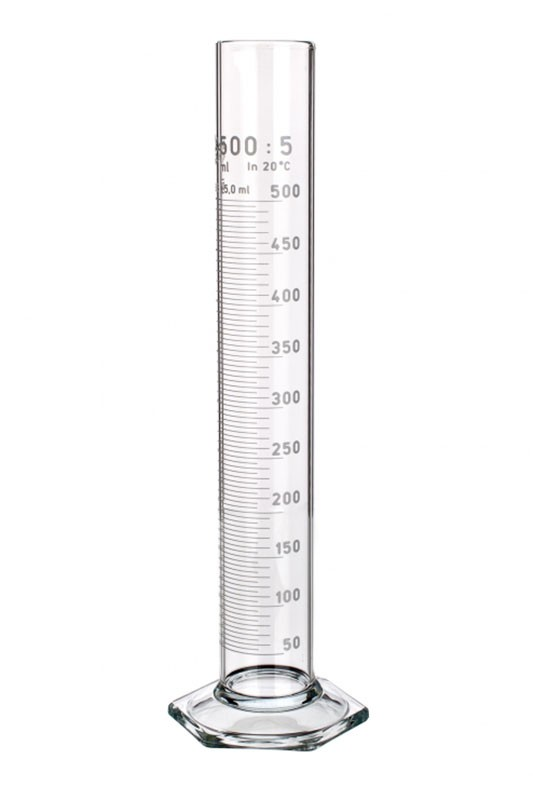
\includegraphics[scale=0.4]{obrazky/odměrný válec.jpg}
    \end{center}
    \caption{Odměrný válec \cite{Odměrný válec}}
\end{figure}
%ZDROJ: https://www.vinarskepotreby.cz/odmerny-valec-1000-ml-sklo.html#gallery

\subsection{Příklad tepelné roztažnosti}
\begin{equation}
\label{objem_kapalina}
    \Delta V = \Delta V_v + \Delta V_e \left[m^3\right]
\end{equation}


\[\Delta V = 0,64 + 1,13 = 13,74 \left[ml\right]\]


\(\Delta V\) ...celkový rozdílový objem

\(\Delta V_{v}\) ...rozdílový objem vody \([m^3]\)

\(\Delta V_{e}\) ...rozdílový objem ethanolu \([m^3]\)


\begin{equation}
%\label{objem_kapalina}
    \Delta V_v = \frac{p_v}{100} \cdot V_0 \cdot \beta_v \cdot (t_1 - t_0)
\end{equation}

\[\Delta V_v = \frac{20}{100} \cdot 1 \cdot  2,14 \cdot 10^{-4} \cdot (20 - 5) = 0,64 \left[ml\right]\]

\(p_v\) ...objemový podíl vody \([\%]\) 

\(V_0\) ...počáteční objem lihoviny \([m^3]\)

\(\beta_v\) ...součinitel objemové teplotní roztažnosti vody \([\frac{m^3}{m^3 \cdot ^\circ C}]\)

\(t_1\) ...koncová teplota \([^\circ C]\)

\(t_0\) ...počáteční teplota \([^\circ C]\)

\begin{equation}
    \Delta V_e = \frac{p_e}{100} \cdot V_0 \cdot \beta_e \cdot (t_1 - t_0)\left[m^3\right] \label{objem_kapalina}
\end{equation}

\[\Delta V_e = \frac{80}{100} \cdot 1 \cdot  1,09 \cdot 10^{-3} \cdot (20 - 5) = 13,1 \left[ml\right]\]

\(p_e\) ...objemový podíl ethalonu(alkoholu) \([\%]\) 

\(\beta_e\) ...součinitel objemové teplotní roztažnosti ethalonu \([\frac{m^3}{m^3 \cdot ^\circ C}]\)




\section{Odměrné válce na alkohol}
\label{valec_na_alkohol}

%Ne příliš moc využívanou alternativou jsou válce
%Nepříliš využívaná metoda, zato mnohem efektivnější od klasického válce, kde je nutno alkohol přelévat, zde nám stačí jen láhev s alkoholem položit do středu válce a sledovat stupnici pro měřený alkohol.\\
Nepříliš využívaná metoda, zato mnohem efektivnější od klasického válce jsou odměrné válce na alkohol. Válec obsahuje několik stupnic, obvykle kolem 40, pro různé destiláty. Láhev alkoholu přiložíme k patřičné stupnici a sledujeme rysku, které odpovídá výška hladiny. Tato hodnota je rovna zbytkovému objemu v láhvi. Výhodou této metody je absence přelévání alkoholu.\\

%Lahev alkoholu přiložíme k patřičné stupnici a jaké hodnotě na stupnici od hladiny
%hodnota na stupnici, které je rovna výška hladiny je rovna zbytkovému objemu v láhvi

%Lahev alkoholu prilozime k patricne stupnici a sledujeme rysku, které odpovídá výška hladiny. Tato hodnota je rovna zbytkovému objemu v láhvi. Výhodou této metody je absence přelévání alkoholu.

\textbf{Výhody}
\begin{itemize}
    \item Cenová dostupnost\\
\end{itemize}

\textbf{Nevýhody}
\begin{itemize}
    %\item \textbf{Časově nákladné}
    \item Válec nemusí obsahovat stupnici s požadovaným alkoholem
    \item Změna tvaru láhve - Pokud výrobce alkoholu změní tvar láhve je nutné kupovat nový válec s novou stupnicí
 %(Nový alkohol - pokud v podniku přibide nový destilát k prodeji je nutné koupit válec...)
    \item Přesnost je závislá na teplotě kapaliny
    %\item Nižší přesnost měření\\\\\\\\\\\\\\\\\\
\end{itemize}

\begin{figure}[H]
    \begin{center}
        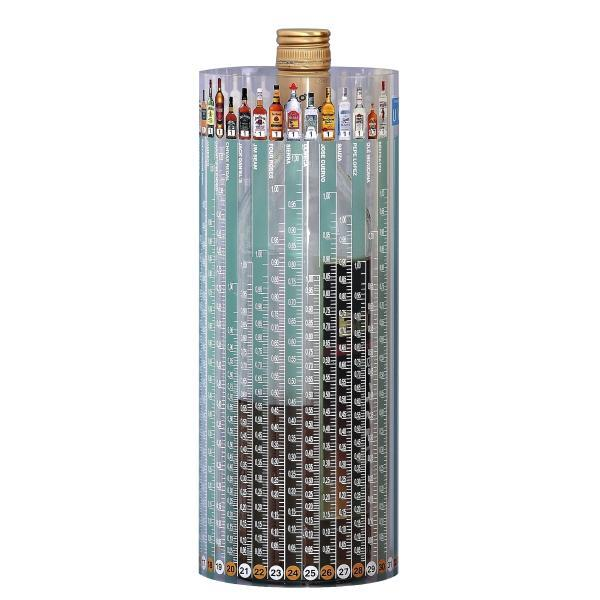
\includegraphics[scale=0.35]{obrazky/odměrný válec na alkohol.jpg}
    \end{center}
    \caption{Odměrný válec na alkohol \cite{Odměrný válec na alkohol}}
\end{figure}

%%Nevyhody:
%zmena tvaru lahve - nutno kupovat nový válec s novou stupnicí
%nepresná hodnota meření

\section{Váhy}
%%foto - mozna
%%Princip přepočtu/výpočtu je podrobneji rozebrán/vice zminen v kapitole [...]

Jedná se o chytré váhy, které na základě databáze s klíčovými daty jsou schopny přepočítat hmotnost měřeného destilátu na jeho objem. 
%Tato problematika je podrobněji rozebrána v kapitole č.3.

Mezi tyto váhy spadá i navrhovaný měřicí systém, který má za úkol inovovat dosavadní měřicí metody. Jeho funkcionalita je více rozebrána v následujících kapitolách. Mezi hlavní nevýhody z pohledu uživatele patří: vysoká pořizovací cena, nutnost jednou za čas kalibrovat váhu a popřípadě doplnění stávající databáze o chybějící destiláty.
%(Databáze je zpravidla rozsáhlá a pokrývá veškeré běžně dostupné destiláty).

%...Toto není nutné pokud datábaze je rozsáhlá a pokrývá i ). více... a v případě méně známých destilátů jejich doplnění do databáze váhy.

%Existuje na světě pár společností vyvíjející váhy se stejným účelem. Bohužel jejich využití v praxi je téměř nulové z důvodu neznalosti existence těchto vah a vysoké ceny. Existuji zjednodušené řešení, kdy se využije običejná váha a aplikace pro výpočet objemu, do které se ručně zadá hmotnost destilátu.

%\section{Porovnání}
%
%Válce činí výhodné pouze jedna věc a to pořizovací cena v opačném případě se jedná o velice neefetivní způsob měření. Přes časové a finanční náklady je stále využívána, protože inventura v podnicích není laboratorní...
%
%Měření zbytkového objemu alkoholu v HoReCa podnicích není záležitostí laboratorního výzkumu tedy požadavky na přesnost jsou minimální, klíčovým fakorem je délka/doba inventury.